The relative two-dimensional spatial coordinates in the plane of the
imaging sensor are known given the size and number of its pixels.  The
absolute three-dimensional coordinates with respect to the scattering spot
are more difficult to assess.  The way in which the experiment is
constructed makes it difficult to accurately measure the distance between
the imaging sensor and the focal spot.  However, with knowledge of the
angle in which the sensor is tilted, the focal spot-sensor distance can be extracted
\textit{a posteriori} from measuring the shape of the light falling on the
sensor.
\begin{figure}[ht]
\centering
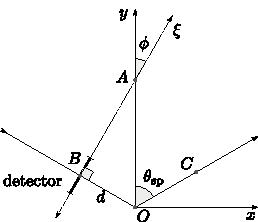
\includegraphics[keepaspectratio,scale=1.25]{figures/hyperbolageoa.pdf}
\caption{Geometry for determining the sensor distance $d$.}
\label{fig:propgeo}
\end{figure}

Consider the experimental geometry shown in \Figure{fig:experimentalsetup}.
Light from scattered SPPs emanates as a cone and is imaged by a planar
sensor.  The light pattern on the sensor is by definition a conic section,
with the re-radiated SPP light as the cone and the sensor as the cutting
plane.  Consequently, the shape of the light on the sensor will be either a
circle, an ellipse, a parabola, or a hyperbola.  In the experimental setup,
the sensor is accordingly fixed orthogonal to the SPP cone.

The geometrical situation is depicted in \Figure{fig:propgeo}.  SPPs
scatter into the far field from point $O$ at an angle $\thetasp$.  The
detector, which has a finite transverse length, is at $B$ and is orthogonal
to $\overline{OB}$ at an angle $\phi=\pi/2-\thetasp$ with respect to the
normal vector from the prism surface $\overline{OA}$.  Because
$\phi<\thetasp$ and $\thetasp>\pi/2$, lines $\overline{BA}$ and
$\overline{OC}$ never intersect. The resulting light pattern on the sensor is a hyperbola.  It is
then relevant to determine, given the parameters of the hyperbolic section,
the distance between the focal spot and the sensor, the line
$\overline{OB}$ with length $d$.

The coordinates of the sensor are represented as $(\xi,y)$, with the
following relationships
\begin{align}
x &= \xi \cos \thetasp \label{eqn:conic01a} \\
r &= \left(d \sec \thetasp + \xi \sin \thetasp\right) \tan\thetasp \label{eqn:conic01b}
\end{align}
and
\begin{equation}
x^2+y^2=r^2.
\label{eqn:conic01c}
\end{equation}
Note $d \sec\thetasp$ is the length of $\overline{OA}$.
\Equation{eqn:conic01b} and \Equation{eqn:conic01c} can be combined to obtain
\begin{equation}
\xi^2 \left(\cos ^2\thetasp-\sin ^2\thetasp \tan
^2\thetasp\right)+2 \xi d \tan ^3\thetasp+y^2=d^2 \tan
^2\thetasp \sec ^2\thetasp,
\end{equation}
which, after a bit of algebra, can be solved for $\xi$, taking
the positive root
\begin{equation}
\xi(y) = \frac{4 \sqrt{2} \sqrt{-2 y^2 \cos 2 \thetasp  \cos ^6\thetasp +d^2
\cos ^6\thetasp -d^2 \cos 2 \thetasp  \cos^6\thetasp}-2 d \sin 2 \thetasp
+d \sin 4 \thetasp }{2 \left(2 \cos 2 \thetasp +\cos 4 \thetasp +1\right)}
\label{eqn:conic02}
\end{equation}

To find the offset, the above minimum is solved to find $\xi(y=0) = 4 d
\sec\thetasp$, and subtracted from \Equation{eqn:conic02}.  The remaining
equation is then solved for $d$,
\begin{align}
d =& \Biggl(-4 \sqrt{2} \Bigl(\delta^2 \sin ^2\thetasp \cos
^4\thetasp+\delta^2 \sin ^2\thetasp \cos \thetasp \cos ^4\thetasp-4 y^2 \nonumber \\
   & \sin ^2\thetasp \cos ^5\thetasp-6 y^2 \sin ^2\thetasp
     \cos ^4\thetasp-16 y^2 \sin ^2\thetasp \cos \thetasp \nonumber \\
  & \cos ^4\thetasp+4 y^2 \sin ^2\thetasp \cos \thetasp
    \cos ^4\thetasp-8 y^2 \sin ^2\thetasp \cos \thetasp \cos
    ^4\thetasp\Bigr)^{1/2} \nonumber \\
&-2 \delta\sin \thetasp-4 \delta \sin 3 \thetasp+\delta  \sin \thetasp-4 \delta \sin \thetasp\Biggr) \nonumber \\
&\cdot\Bigl(4 \left(2 \cos \thetasp+3 \cos \thetasp-3 \cos \thetasp+\cos 5
\thetasp-2 \cos \thetasp-1\right)\Bigr)^{-1}.
\end{align}
where $\delta$ is the distance the cone extends at the coordinate $y$.
By following the aforementioned procedure, given the dimensions of the pixels on the imaging sensor, $d$
can be determined.  Once $d$ is known, the absolute coordinates $(x,y,z)$ of the
sensor are given by
\begin{equation}
  \begin{pmatrix}
          x\\
          y\\
          z
  \end{pmatrix}
  =
  \begin{pmatrix}
          x^\prime \cos\thetasp + d \sin\thetasp\\
          y^\prime \\
          d \cos\thetasp - x^\prime \sin\thetasp,\\
  \end{pmatrix}
\label{eqn:sensorcoordinates}
\end{equation}
where $x^\prime$ and $y^\prime$ are the local coordinates of the sensor
with $(0,0)$ as its origin.
